\documentclass{article}
 
\usepackage{tikz}
\usepackage{hyperref}
\usepackage{xcolor}
\usepackage{breakurl}
\usepackage{graphicx}
\usepackage{float}
\usepackage[margin=1in]{geometry}


\title{Data Mining Hospital Readmissions and Mortality Rates using Multiagent Random Forest}
\author{Andrew Berry}
\date{\today}

\begin{document}
\maketitle

I pledge my honor that I have neither given nor received any unauthorized aid on this work.

\section{Introduction}
\par
My project attempts to use machine learning with multiple learning agents to analyze a hospital dataset from data.gov\textsuperscript{1} to determine whether, given metrics for readmission and death of patients due to various medical conditions and diseases, we can predict (with reasonable accuracy) where the hospital is located within the United States. This is measured as the percentage of states that the system correctly chooses for the hospitals in the test set, and additionally as a similar percentage for geographic regions. In the event this project fails to produce an adequately accurate classification system from this approach, the hope is that it at least illustrates (using the same multi-agent learning environment) that there is some statistically significant correlation between these readmission and death metrics and geographic location.

\section{System Description}
\par
This project was built entirely in python, using the libraries pandas, scikit-learn, and SPADE primarily. 

\par
Pandas\textsuperscript{2} is a python library for data analysis which allows efficient data manipulation through data structures such as the pandas dataframe. The original hospital dataset contained columns for measure ID and score. My system used pandas dataframe functions to pivot these out to 14 measure columns such that we have one row per hospital. This allows me to specify the 14 columns as the columns for the classification algorithm to consider when training the random forest classifier. This pivoted approach was used because it intuitively seemed that having 14 different columns to use in training the algorithm would clearly produce a more appropriate tree structure than just using 2 columns (that is, the measure name and measure value in the non-pivoted set). 

\par
Scikit-learn\textsuperscript{3} is a library that contains efficient implementations of various data mining/machine learning algorithms. The system I created uses the randomForestClassifier class from scikit-learn to perform classification over the test dataset to predict values for state and region. 

\par
SPADE\textsuperscript{4} is a python library for implementing multiagent systems. It comes with FIPA-ACL communication functionality built into its agent behaviours (using the XMPP/jabber communication protocol). My project incorporated these abilities to allow multiple agents to learn over the dataset and communicate their predictions to each other.

\par
My system implements an example of the distributed artificial intelligence concept of centralized multiagent learning. Centralized multiagent learning is multiagent learning in which the learning process is isolated from influence of other agents in the system. In my system, although the agents convey their solutions to each other, the learning itself does not include agent intaraction. Each agent learns independently of the others and the listener agent considers the input of all other agents when making a choice. 
\par The system also incorporates communication between the agents in the system. SPADE comes standard with FIPA-ACL message sending and receiving capabilities for the basic agent class, from which my TalkerAgent and ListenerAgent classes inherit.
\par The original project description and following updates described a system of $n$ agents in which there is one initial ``talker'' agent, $n-2$ ``talker/listener'' agents, and finally one ``listener'' agent at the end of the line. The system was kicked off by starting the ``talker,'' having it calculate its predictions, tell those to the first ``talker/listener'', who weighed them against its own choices, passing its final answer to the next agent in the line, until program execution arrived at the final ``listener'' agent which gave the final answer of the program. 
\par This approach (which I have been calling the ``linked-list'' approach) was later revised into one which used a star-shaped agent graph in which there are $n-1$ ``talker'' agents, which all send their predictions to a single ``listener'' agent (an agent organization scheme which I will refer to as the ``star-graph'' approach hereafter). This reduction of complexity (via removing the need for any agents to talk and listen simulaneously) helped allow me to run simulations with more agents than I previously could in the linked list model.

 \section{Experimental Design}

\par This project was undertaken in the hope of finding that state/region of a hospital could be (somewhat) accurately predicted by a multiagent learning system which was trained over readmission and death rates for various conditions at other hospitals in the United States. 

\par My initial (weakest) hypothesis ($h_{1}$) was that a there exists correlation between hospital metrics and geographic location within the United States. This correlation was expected to be strong enough that my program should be able to predict state and region with better-than-random accuracy. The second hypothesis ($h_{2}$) was that introducing multiple agents to the classification problem should provide additional flexibility to the decision process and allow the system to further improve prediction capability.

\par Decision tree classification allows two different methods for determining the accuracy of its classifications: Gini impurity and entropy\textsuperscript{5}. Each of these values represents how ``mixed'' a set is, and thus the goal of the decision tree classification algorithm is to choose splits of data that minimize these quantities. Since random forest is an extension of decision tree learning, the scikit-learn RandomForestClassifier class allows choice between these two measurements as well. My experimental setup contains 2 different experiments, in which I vary the number of agents in the system ($n$), the number of trees per forest ($k$), and the metric used to determine the ``mixed-ness'' of the set($\mu$). While these quantities vary between the experiments, the size of the training set (and thus the size of the test set) are fixed at 4445 and 100, respectively. This means that the number of correct guesses for each trial in each experiment can be taken at face value to represent a percentage correctness, since the total number of guesses made is 100 in all cases.

\section{Experimental Results}

%\par Specific details for each experiment
\par The first experiment run used 30 agents, each with a classifier of approximately 100 trees (number of trees was a randomly chosen number from a sequence going from 60 to 140 incrementing by 10), using Gini impurity as the mixed measure. This experiment was run for 20 trials. Some graphical results of the trials of this first experiment are shown in figures 1 and 2. 
\par Note: For all figures in this paper, ``S'' indicates that the measure applies to states, ``R'' indicates that the measure applies to regions, ``Ind'' indicates that the measure corresponds to predictions made independently by an agent (ignoring other agents' input), ``Crwd'' indicates that the measure corresponds to ``crowdsourced'' prediction based on the predictions of other agents, and ``Improve'' indicates measures that are defined as $Crwd-Ind$; that is, how much the accuracy of prediction improved when moving from an independent to a crowdsourced prediction model.
\par Examining figures 1 and 2, we can see that there is no consistently present improvement that is gained in each trial by switching from independent to crowdsourced information, but looking at the averages we do see a small improvement over average accuracy of prediction for both states and regions. Figure 2 shows us just how small this improvement is: less than 1\% for states and between 1 and 2\% for regions. 

\begin{figure}[H]
		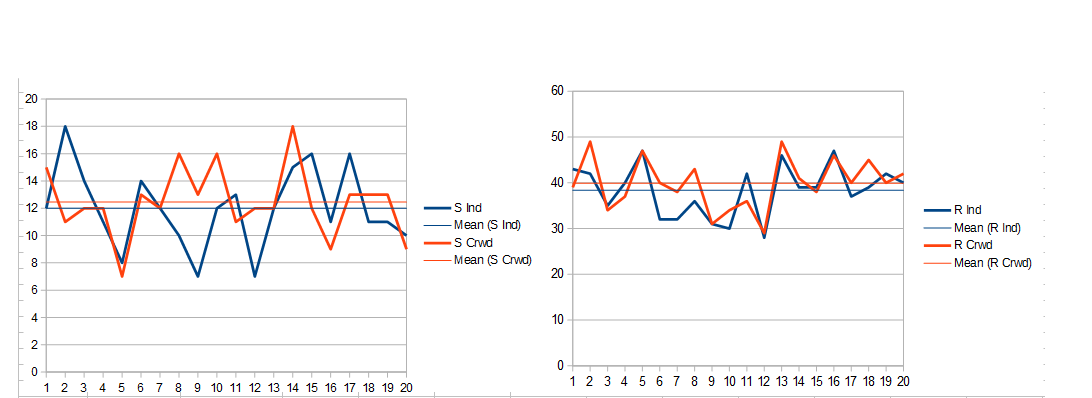
\includegraphics[width=\textwidth]{e1_comparative}
		\caption{Experiment 1 State and Region Comparisons}
\end{figure}

\begin{figure}[H]
	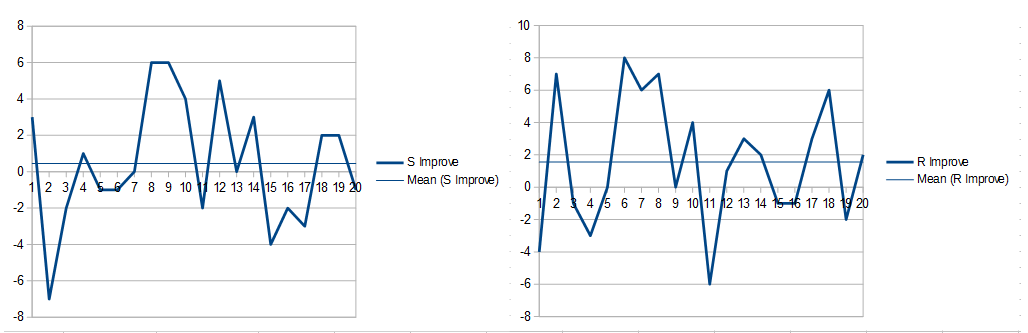
\includegraphics[width=\textwidth]{e1_improvement}
	\caption{Experiment 1 State and Region Improvement via Agent Collaboration}
\end{figure}

\par The second experiment run used 10 agents, each whith a classifier of approximately 100 trees (number of trees was a randomly chosen number from 60 to 140 as in experiment 1), using entropy as the mixed measure instead of Gini impurity. This experiment was run for 20 trials. Some graphical results of the trials of this second experiment are shown in figures 3 and 4.
\par Switching from Gini impurity to entropy as the mix measure was somewhat problematic to the runtime of the system, hence the dramatic reduction in the number of agents in the second experiment. This reduction in agent population makes it more difficult to draw an accurate conclusion of how the system performs in this experiment. Initial review of figures 3 and 4 appear to show that this experiment offered better improvement as far as state classification is concerned, but interestingly performed poorly enough in one trial of region classification that it brought the average improvement for regions in the experiment below 0, effectively making it seem that the agent is worse off for having considered other agents' opinions.
\par The results of experiment 1 reveal that $h_{1}$ appears to hold true. In the case of classifying hospitals to particular US states, one would expect a random choice of state to give a correct answer about $2\%$ of the time. Given that I have divided the United States into 6 regions, one would also expect a random choice of region to give a correct answer about $16.\overline{6}\%$ of the time. In all cases, whether state classification or region classification, educated or uneducated choice, gini impurity or entropy mixed measure, the system outperforms random guessing at classifying rows of data. This reveals that there does exist a correlation between the hospital metrics and their location. I feel a fairly high degree of confidence saying that $h_{1}$ is supported by these experimental results.
\par For $h_{2}$, I cannot as readily accept that it has been supported, but it appears that there may be some promise to the inter-agent communication approach. The averages seem to suggest that $h_{2}$ is somewhat supported, but looking at some of the individual trials in which the ``educated'' choice gave significantly worse performance than the independent one, it begs the question of whether these results were the product of a particularly lucky set of trials.

\begin{figure}[H]
	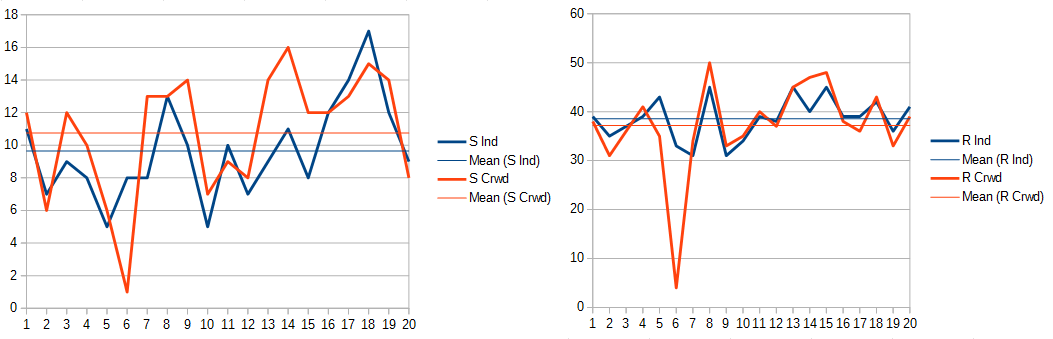
\includegraphics[width=\textwidth]{e2_comparative}
	\caption{Experiment 2 State and Region Comparisons}
\end{figure}

\begin{figure}[H]
	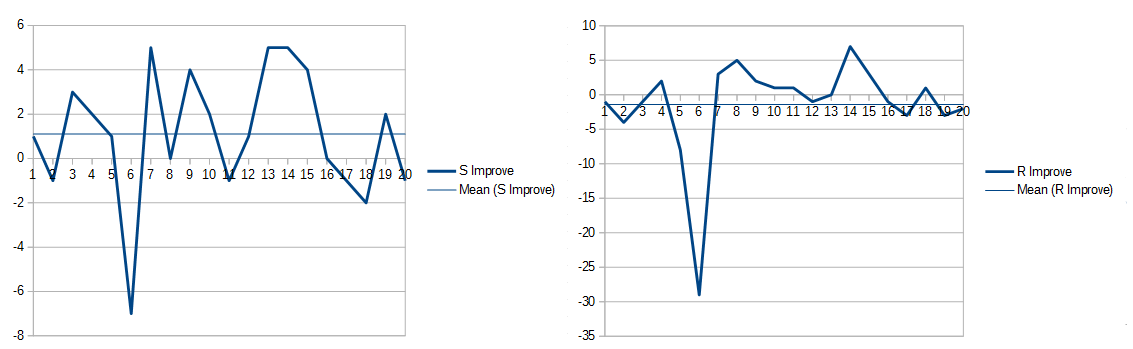
\includegraphics[width=\textwidth]{e2_improvement}
	\caption{Experiment 2 State and Region Improvement via Agent Collaboration}
\end{figure}



\par The results of experiment 2 still appear to support $h_{1}$, since all but one trial still produced better classification than random guessing would have.
\par In regard to $h_{2}$, this experiment seems to come closer to undermining the likelihood that inter-agent communication can significantly improve accuracy of classifications, at least in the case of regions. The states classification results were no worse than those in the first experiment and lend some small amount of support to the hypothesis.


%\par Graphs and tables?

%\par Specific aspects of the experiments that led to results?

\section{Discussion}

%\par Overarching discussion of results across all experiments

\par Although the number of trials was small and not all trials resulted in improved utility, the results presented seem to have some promise. If the experimental results are viewed as separated into four categories (Gini-States,Gini-Regions,Entropy-States,Entropy-Regions), three of the four showed an improvement to the classification capabilities of the system when multiple agents' predictions are considered in choosing the final state/region for a row. However, it is important to bear in mind that the average improvement of the classification is meager compared to improvements that could possibly be acquired through running the simulation with one agent that has a much higher number of trees in the random forest.


%\par Final Para: Projects process... were milestones met? Everything accomplished? What would you change if starting from square one?
\par In regard to the project process for this course, I kept to the schedule outlined in the initial project summary during the project updates throughout the semester. However, a significant volume of work was still required toward the end of the semester such that the most intense efforts were concentrated in late November. I would consider my project overall moderately successful in that it implemented a machine learning algorithm in a multiagent environment and was able to produce results, even if those results were less promising than originally hoped. If I were to re-attempt this project from the beginning, I would have tried to skew the workload more toward the earlier part of the semester to give myself more time to work out kinks in the program execution (performance issues, etc.). I also would make more use of office hours to ensure that the project stays on track better, since many of the late-stage improvements I have incorporated were discovered during the project demonstration phase.

\section{Future Work}

%\par If future work was to occur, what would you do? Why make those changes?
\par It is unclear at this point whether the process fails to reliably produce systematic improvements due to the nature of the system itself, the limited memory capacity of the machine used, or the lack of a strong correlation between the columns in the hospital domain. Future considerations could be to run these experiments on a computer with more memory, and run it on more varied subject areas that are already understood to have a strong relationship between training columns and predicted classifications. This would allow a more even-handed, accurate view of whether a multiagent extension of the random forest algorithm improves its ability to classify.

\section{Conclusions}

%Brief summary
\par This project has sought to show that readmission and death rates for various medical conditions can serve as a guideline for predicting where in the United States a hospital is located using a multiagent learning system. The success rate was nothing groundbreaking but it has been determined that there does exist a correlation between these.

\section{References}

{[}1{]} Readmissions and Deaths - Hospital. https://catalog.data.gov/dataset/readmissions-and-deaths-hospital \\
{[}2{]} Pandas - Python Data Analysis Library. http://pandas.pydata.org/ \\
{[}3{]} Scikit-learn - Machine Learning in Python. http://scikit-learn.org/stable/ \\
{[}4{]} SPADE - Smart Python multi-Agent Development Environment. https://pypi.python.org/pypi/SPADE \\
{[}5{]} T. Segaran, \textit{Programming Collective Intelligence}. O'Reilly Media Inc., 2007 \\





\end{document}
